\documentclass{standalone}
\usepackage{tikz}

\usetikzlibrary{calc,math}


\begin{document}

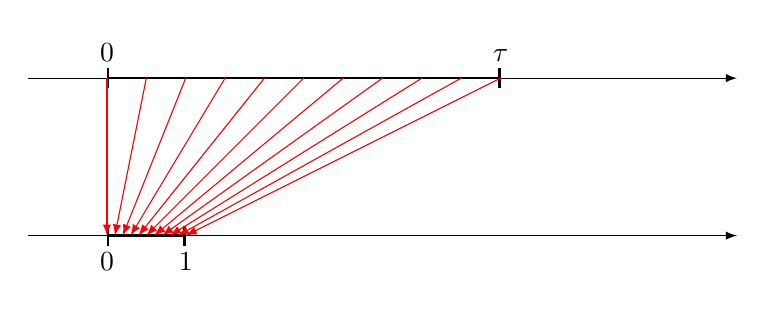
\begin{tikzpicture}
  \draw[thin,-latex] (-1,0) -- (8,0);
  \draw[|-|,thick] (0,0) node[above,inner ysep=2mm] {0} -- (5,0) node[above,inner ysep=2mm] {$\tau$};
  \draw[thin,-latex] (-1,-2) -- (8,-2);
  \draw[|-|,thick] (0,-2) node[below,inner ysep=2mm] {0} -- ++(1,0) node[below,inner ysep=2mm] {1};

  \foreach \x in {0,0.1,...,1.01} {
    \tikzmath{
      real \y;
      \y = \x * 5;
    }
    \draw[red,-latex] (\y,0) -- (\x,-2);
  }
\end{tikzpicture}

\end{document}
